\documentclass{beamer}
\usepackage[utf8x]{inputenc}
%\usepackage{default}
\usepackage{verbatim}
\usepackage{graphicx}
\usepackage{listings}

\title{Combining Roborescue and XABSL}
\subtitle{Final Presentation}
\author{Maarten de Waard}
\institute{UvA}
\usetheme{Berkeley}
\newcommand{\slide}[2]
{
\begin{frame}
\frametitle{#1} 

#2

\end{frame}
}

\begin{document}
{
\usebackgroundtemplate{
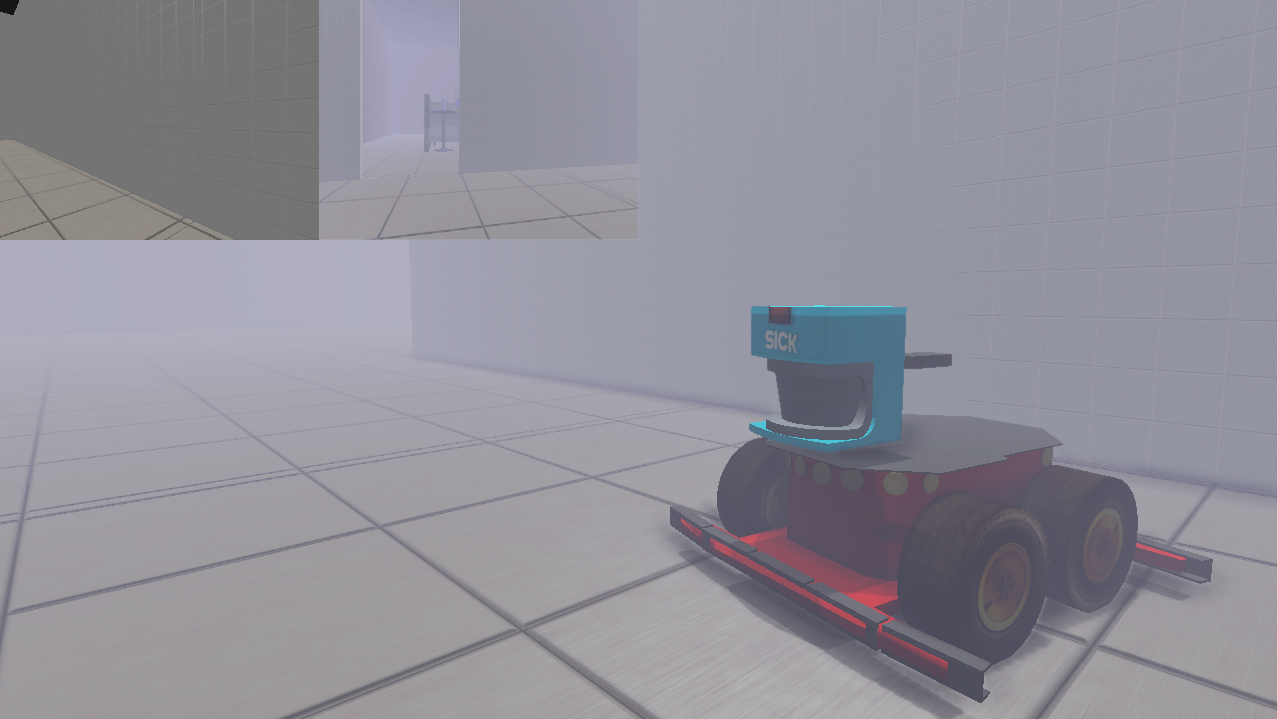
\includegraphics[width=\paperwidth, height=\paperheight]{interface}
}
\begin{frame}
\titlepage
\end{frame}
}

\begin{frame}
\tableofcontents
\end{frame}

\section{Recap}
\slide{Recap}
{
    To freshen your memories, a short summary of my research and my goal:
    \begin{itemize}
        \item UsarCommander - the program used by the UvA Rescue team in the
        RoboCup
        \item XABSL - eXtended Agent Behavior Specification Language
        \item The combination - A thriving combination of UvA's Rescue research and Germany's winning robotic soccer team.
    \end{itemize}
}

\section{Challenges}
\subsection{VB and C++}
\slide{Visual Basic and C++}
{
    \begin{columns}
    \column{.5\textwidth}
    Problem: The XABSL Engine written in C++, UsarCommander in Visual Basic
    
    Solution: create a Dynamic Link Library (DLL) containing XABSL.
    Approach:
    \begin{itemize}
        \item Create runnable DLL, and run it from Visual Basic
        \item Create a C++ program implementing the needed XABSL files
        \item Create DLL from the C++ program.
    \end{itemize}
    \column{.5\textwidth}
    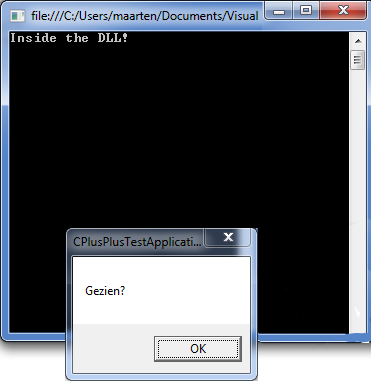
\includegraphics[width=\columnwidth]{dll.png}
    \end{columns}
}
\slide{Visual Basic and C++: The problems}
{
    \begin{itemize}
        \item No experience: Creating a DLL from an entire framework is
        different than a `Hello World' DLL.
        \item Cryptical errors
    \end{itemize}
    \begin{block}{The error:}
    \texttt{error LNK2019: unresolved external symbol "public: void \_\_thiscall
    xabsl::Parameters::registerDecimal(char const *,double \&)"
    (?registerDecimal@Parameters@xabsl@@QAEXPBDAAN@Z) referenced in function
    "public: virtual void \_\_thiscall TestBehavior::registerParameters(void)"
    (?registerParameters@TestBehavior@@UAEXXZ)}
    \end{block}
}
\subsection{JXABSL Engine}
\slide{JXABSL}
{
    Luckily, there was an alternative to the C++ engine:
    \begin{itemize}
        \item XABSL Engine programmed in Java
        \item Little documentation
        \item Impossible to create direct connection to VB
    \end{itemize}
    Solution:\\
    Socket connection between JXabsl and UsarCommander
}
\section{Approach}
\subsection{JXI}
\slide{JavaXabslImplementation}
{
    \begin{itemize}
        \item Framework providing all XABSL-possibilities over a socket
        connection 
        \item Easier to use than JXABSL
        \item Modular
    \end{itemize}
}
\slide{Information flow}
{
    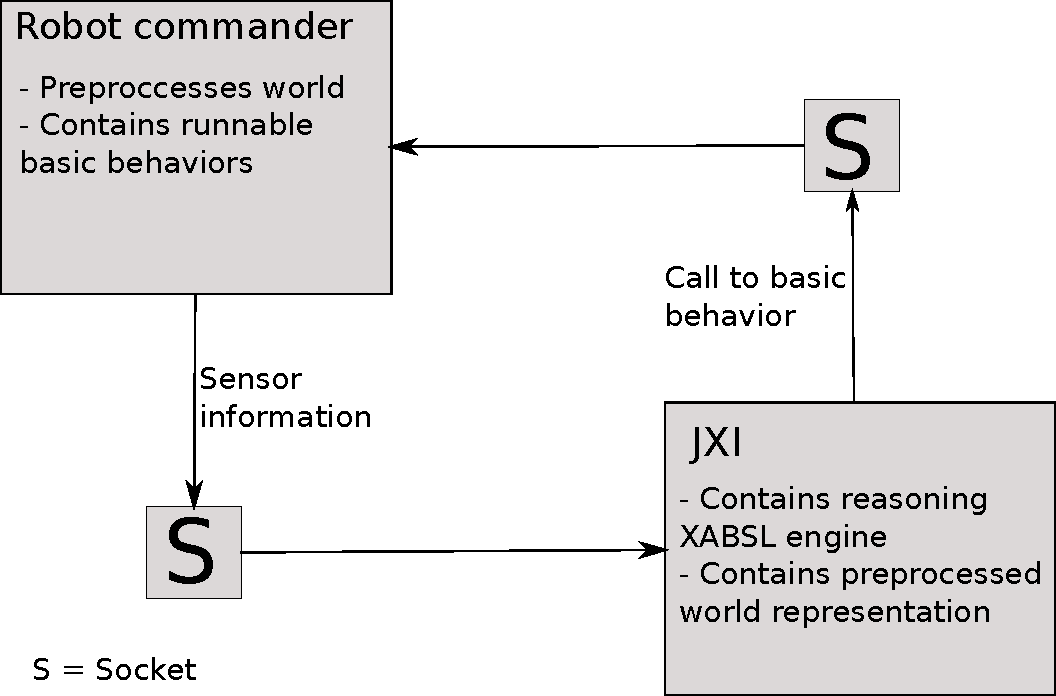
\includegraphics[height=.8\textheight]{informationFlow.pdf}
}
\section{Results}
\slide{XABSL behavior}
{
    Two simple behaviors were created:
    \begin{itemize}
        \item Drive\_circle:
        \begin{itemize}
           \item Makes the robot autonomously drive a circle
        \end{itemize}
        \item Walk\_corridor
        \begin{itemize}
            \item Makes the robot traverse though a corridor without bumping
            into anything
        \end{itemize}
    \end{itemize}
}
\lstset{frame=single, numbers=left,
    language=java,
      keywordstyle=\bfseries,          % keyword style
      morekeywords={include, agent},
      basicstyle=\tiny
    }
\begin{frame}[fragile]
\frametitle{Code for walk\_corridor}
    \lstinputlisting[tabsize=2]{walk_corridor_option.xabsl}
\end{frame}

\begin{frame}[fragile]
\frametitle{Code for walk\_corridor}
    \lstinputlisting[tabsize=2]{walk_corridor_states.xabsl}
\end{frame}
\slide{Generated option graph}
{
    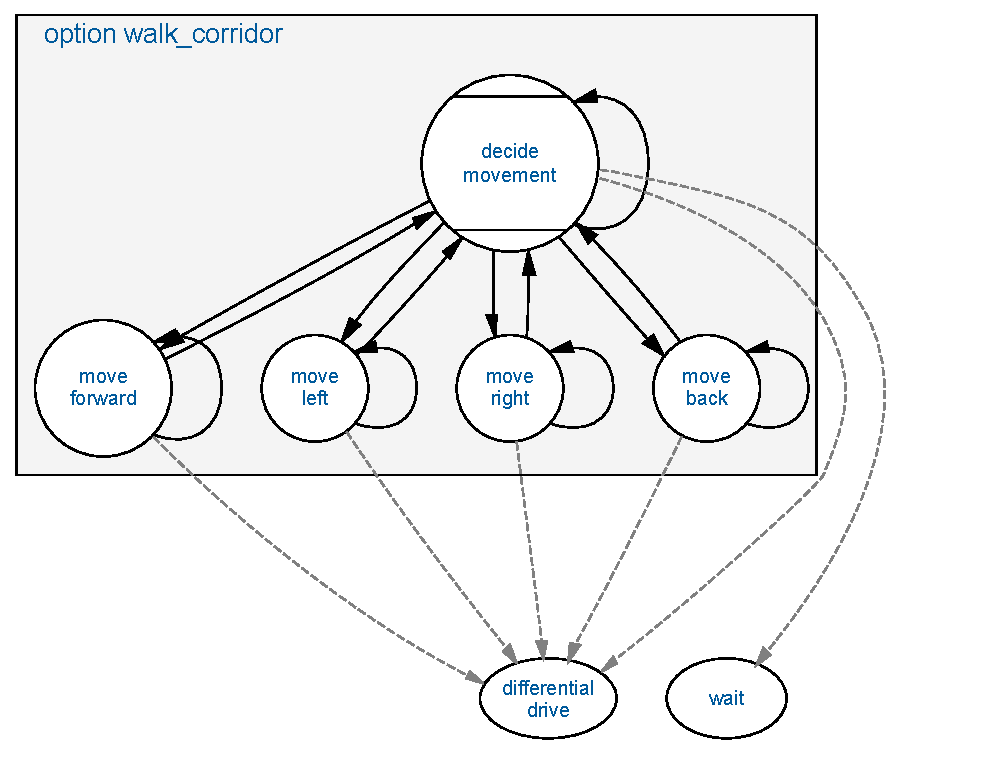
\includegraphics[width=.9\textwidth]{option_walk_corridor.pdf}
}
\section{Demo}
\slide{Demo}
{
    A film of the robot turning 360 degrees, powered by JXI!
    \url{http://www.youtube.com/watch?v=0ixdA-mzoCg&feature=youtu.be}
}
\section{Conclusion}
\slide{Conclusion}
{
    Good points:
    \begin{itemize}
        \item In theory, everything works.
        \item JXI can be combined with any program, because of its use of
        sockets
        \item The framework offers a lot of possibilities
        \item The framework offers easier understanding and implementing of XABSL
    \end{itemize}
    Possible improvements:
    \begin{itemize}
        \item The framework currently only works with one robot
        \item More complex behaviors could be implemented, to test the
        frameworks abilities
        \item Fixing the bugs in UsarCommander would seriously increase speed of
        the complete program.
    \end{itemize}
}





\section{}
\slide{Questions}
{}



\end{document}
